\documentclass[10pt]{article} % For LaTeX2e
%\usepackage{nips13submit_e,times}
\usepackage{hyperref}
\usepackage{url}
\usepackage[round]{natbib}
\usepackage{amsmath}
\usepackage{graphicx}
\usepackage[margin=1in]{geometry}
\usepackage{subfig}
\usepackage{threeparttable}
\usepackage{rotating}
\usepackage{xcolor}
\usepackage[textsize=footnotesize, colorinlistoftodos, textwidth=4cm, obeyDraft]{todonotes}
 \usepackage[bottom, multiple]{footmisc} 
\newcommand{\cfbox}[2]{%
    \colorlet{currentcolor}{.}%
    {\color{#1}%
    \fbox{\color{currentcolor}#2}}%
}
%\documentstyle[nips13submit_09,times,art10]{article} % For LaTeX 2.09


\title{Can Monitoring and Citations Make Food Safer?}

\author{
Jason Huang \\
Department of Economics\\
Stanford University\\
Stanford, CA 94305 \\
\texttt{jhuang99@stanford.edu} \\
}

% The \author macro works with any number of authors. There are two commands
% used to separate the names and addresses of multiple authors: \And and \AND.
%
% Using \And between authors leaves it to \LaTeX{} to determine where to break
% the lines. Using \AND forces a linebreak at that point. So, if \LaTeX{}
% puts 3 of 4 authors names on the first line, and the last on the second
% line, try using \AND instead of \And before the third author name.

\newcommand{\fix}{\marginpar{FIX}}
\newcommand{\new}{\marginpar{NEW}}

%\nipsfinalcopy % Uncomment for camera-ready version

\begin{document}


\maketitle

\begin{abstract}

Many local and state governments conduct regular health inspections on retail food establishments to ensure proper hygiene standards, and they hand out citations when the standards are not upheld. But how effective are these citations in incentivizing the restaurants to improve their sanitation practices? By analyzing food inspection data from New York City's Department of Health and Mental Hygiene, along with 311 complaint calls, I examine how restaurants respond to citations given out during regular food inspections. I find that more citations leads to better subsequent inspections. I also find that the establishments not only address the areas for which they received citations but also improve in other areas, suggesting complementarity across multiple dimensions of cleanliness. Furthermore, I find that consumers also respond to these improved sanitation conditions by making 311 complaint calls less frequently. To deal with the endogeneity of the inspection results, I exploit the random assignments of inspectors and construct inspector-specific measures of stringency as an instrumental variable. I find that this variable is highly predictive of not only the total scores but also the specific violations that are cited, despite the random assignment process that results in similar restaurant characteristics across inspectors. 

\end{abstract}

\section{Introduction}

Food hygiene at restaurants is a great public health concern. The CDC estimates that over 3 million incidents of food-borne illness occur in the US annually, with 60\% of the cases resulting from  dining in restaurants.\footnote{Surveillance for Food borne Disease Outbreaks United States: 2013 Annual Report. Available: https://www.cdc.gov/foodsafety/pdfs/foodborne-disease-outbreaks-annual-report-2013-508c.pdf} Unlike food quality or service, which consumers can easily observe, food sanitation remains opaque to consumers since most diners cannot venture back to the kitchens and monitor the food preparation process. Local health departments have long conducted regular food inspections to ensure that restaurants meet certain hygiene standards. 

This paper estimates the causal impact of NYC's food inspection results on restaurant compliances and customer perceptions, measured by frequencies of 311 complaints calls. Inspection results can potentially influence restaurant behaviors through for two reasons. First one is monetary. The scores determine the letter grades restaurants post on their entrance windows. These grades can influence consumer demand and affect revenues. The second one is behavior. restaurants may improve by learning from previous mistakes through the citations. Restaurants may commit violations not because they are profit maximizing by cutting enough corners to equate the marginal savings with the marginal costs from penalties. Instead, restaurants may be simply making mistakes because of lack of knowledge or experience.\footnote{A potential reason is that scores are directly associated with monetary penalties. Each violation is associated with a fine, and the amount of fine depends on the severity cited by the inspector. However, the amounts of these fines are very small, ranging from 200 to 1000 per violation.} Given that cleanliness is a multi-dimensional task, I examine how the distribution of citations impact the distributions of efforts across these dimensions. In addition, I test whether consumers behaviors respond to changes in restaurant hygiene efforts by measuring the changes in the frequencies of 311 complaint calls to DOHMH.

I find that more citations results in improved outcomes during subsequent inspection results. Receiving an one standard deviation worse overall sanitation score leads to an 0.23 standard deviation improvement in the overall score, a 9 percent increase in probability of earning an A, and 62 percent decrease in probability of being temporarily shutdown for unresolved critical violations during the subsequent inspection. While most of the improvement that a citation caused the restaurant to make is in the same area, citations in some areas led to improvements in other areas. For example, I find that an additional citation in Facility Design led to 0.195 fewer citation in Food Protection, in addition to 0.2 fewer citation in Facility Design. After merging the inspection data with the 311 complaint call data, I find that getting a worse inspection score also leads to fewer complain calls, suggesting that customers also notice the improved sanitation qualities.

Even though understanding how small businesses respond to citations is of interest to academics and policy makers, there is a dearth of studies on this topic. A major empirical challenge is that the variable of interest is endogenous. The inspection results depend on both the effects of monitoring and compliance, and we need to disentangle the two to estimate the causal effect of citations. For example, suppose we find that restaurants that had high numbers of citations tend to have high number of citations in the future. Do more citations lead to worse compliance or do restaurants that did poorly in the past continue to do poorly in the future? This paper uses the random assignment of food inspectors to inspections for restaurants in New York City as an instrumental variable to overcome the endogeneity of inspection results. As different inspectors have different levels of stringencies, the results that restaurants receive are partly determined by chance.\footnote{Other areas of research that have used this random assignments of decision makers to recover causal impacts of include the impact of incarceration on recidivism \citep{bhuller_16}, the effect of disability insurance on labor supply \citep{Maestas_13}, and the impact of foster care system on child outcomes \citep{Doyle_07}.}

A growing literature that complements this paper has focused on the role of transparency, rather than citation and citation, to improve food sanitation and reduce food-borne illness. The first type is certification, or what \cite{Ho_2012} calls targeted transparency. Letter grade system, first introduced in Los Angeles and later adopted by New York City is one example of certification. \cite{jie_leslie_05} and \cite{Simon_05} study the introduction of the grading system in Los Angeles in 1998 and find strong evidence for a decrease in hospitalization for foodborne illnesses in jurisdictions after the enactments of the grading systems. \cite{jie_leslie_05} argue that the reduction is driven by people cooking more at home and eating out less. \cite{Wong_at_el_2015} and \cite{Meltzer_2015} study New York City's food inspection program. They use inspection scores to measure restaurant cleanliness. After finding that improved sanitation scores and lower violation fines followed the reform, they conclude that the reform improved sanitation practices. These papers looks at impact of the overall inspection program while I study the effect of individual inspections. \cite{Filion_Powell_09} document the growing popularities of these grading programs across the globe. The second type of transparency arise from customer reviews. \cite{Luca_13} use Yelp reviews to predict health code violations, and they argue that inspection selection can be optimized based on information from social media. [TODO: Say more about indirect] ]However, sending food inspectors to restaurants for inspections remains as the most direct tool of enforcement, and understanding the impact of these inspections on compliance remains important. Hence, I see this study about monitoring and detection as a complement to instead of a substitute of studies about the role of transparency. 

This paper also relates to a broad literature that studies the connection between government monitoring and compliance. Researchers have explored this issue in other areas such as taxation (\cite{Feinstein_91}, \cite{Kleven_etal_10}, \cite{Gemmell_Ratto_12}), workplace safety \citep{levine_etal_12}, nuclear power plants \citep{Feinstein_89}, and environmental protection \citep{Duflo_Greenstone_14}. While \cite{Jin_Lee_12} and \cite{Jin_Lee_14} also examines the food inspection programs, the two papers focus on the inspectors' behaviors and detection technology. \cite{Jin_Lee_14} provides suggestive reduced form evidence that improved detection technology lowers the probability of food borne disease outbreaks, it does not provide evidence that links inspector behaviors with restaurant compliance, which this paper does.

\section{New York City Food Inspection System}
\label{background}

New York City's DOHMH oversees the food safety program. It sends out food inspectors to restaurants to conduct inspections. Each restaurant receives at least one inspection a year. Starting in 2005, the city implemented a numerical scoring system. It outlined ninety-eight violations, broken into eight categories. Each violation is associated with a range of scores, and the inspector assigns the numerical value that reflects the severity of the violation. For example, a violation 10F for not non-food contact surface improperly constructed is worth from 2 to 5 points, depending on how many of these surfaces the inspector finds.\footnote{See Food Service Establishment Inspection Procedures Handbook: 

http://www1.nyc.gov/assets/doh/downloads/pdf/about/healthcode/health-code-chapter23.pdf. }

Starting in 2010, the sum of the scores were converted to letter grades, A, B, C. A score between 0 to 13 earns an A, between 14 to 27 earns a B, and 28 or above earns a C. The city required the restaurants to post these letter grades on the entrance so that they are clearly visible to the customers. The grading policy also ntroduced dual inspection cycles, which involves the a random initial inspection and a possible re-inspection within a month if the initial inspection results in a letter grade lower than an A. During the time in between the initial inspection and re-inspection, restaurants can either post their assigned letter grade or a sign saying "Grade Pending." The score from re-inspection is then used to determine the letter grade the restaurant posts until the next initial inspection, and the previous initial inspection result has no effect. 

As a result of these letters, ... bunching
\begin{figure}[htbp]
\centering
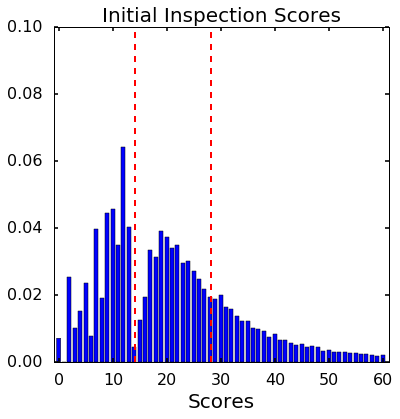
\includegraphics[scale = 0.45]{Figures/init_score.png}
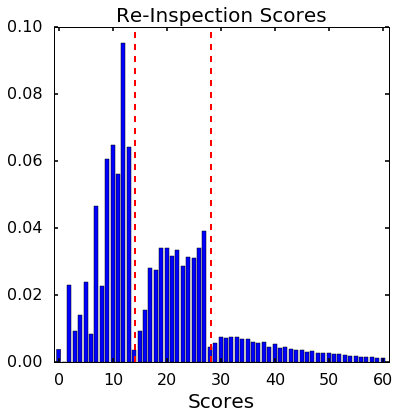
\includegraphics[scale = 0.45]{Figures/re_score.png}
\caption{Score Distribution of Initial Inspections and Re-inspections.}
\label{bunching}
\footnotetext{This figure displays the distribution of inspection scores during initial inspections and re-inspections. The dotted red line represents the 13-14 points and 27-28 thresholds.}
\end{figure}

DOHMH may temporarily close a restaurant for two reasons. The first reason is that the establishment poses a public health hazard that cannot be addressed by the end of the inspections. Such hazard includes issues such hot food not cooked to high enough temperature or cold food not stored at low enough temperature, presence of unpasteurized milk, or harmful noxious gas detected. The second reason is that restaurants receive scores above 28 for three consecutive inspections. If closed, DOHMH immediately posts a closure sign on the window. To reopen, the establishment must submit a written statement to DOHMH that describes the steps it has taken to correct the violations. Then re-opening inspection occurs. The median time between closure and re-opening inspection is 4 days, with 95\% of the cases occurring within 24 days. The establishment can re-open if it passes the re-opening inspection, but it receives its next initial inspection within three months. Repeat violations may prompt DOHMH to shutdown an establishment for longer or permanently. 

\section{Empirical Analysis}
\label{empirical_sec}

\subsection{Stringencies of Inspectors as Instrumental Variable}
\label{IV}

An ideal experimental design to estimate the causal effect of citations on restaurant compliance behavior is to randomly vary the number of citations each restaurant receives. However, inspection results are not random and are potentially correlated with variables, such as the restaurant's management quality or financial health, that are also correlated with restaurant's sanitation quality, regression estimates suffer from omitted variable bias. To address this issue, I exploit the two institutional features of NYC's food inspection program to create a natural experiment. First, according to the staff of DOHMH, inspectors are randomly assigned to restaurant for each inspection to ensure equity. They do not specialize in any particular geography or type of restaurant. Second, the levels of stringencies among the inspectors vary widely, with some inspectors being very strict while other being more lenient. 

To empirically implement this natural experiment, I create an instrumental variable that reflect the level of stringency of each inspector that a restaurant faces during an inspection. Specifically, I define the instrument between restaurant $i$ and inspector $j$ as
\begin{align}
\label{instrument}
    Z_{ij} = \frac{1}{n_{j} - I_{ij}} \left( \sum_{kjtp\neq ijt}  SCORE_{kjt}\right)
\end{align}
where $n_{j}$ is the total number of initial inspections conducted by inspector $j$, $I_{ij}$ is the total number of initial inspections inspector $j$ has conducted at restaurant $i$, and $SCORE_{kjt}$ is the score inspector $j$ gave to restaurant $k$ on date $t$. 

Figure \ref{first_stage_fig} plots the distribution of the inspector average scores. The histogram shows a considerable amount of heterogeneity in terms of inspectors' levels of stringencies.\footnote{See \cite{Feinstein_89}, \cite{Feinstein_91}, and \cite{Macher_11} for additional documentation of inspector heterogeneity pertaining to IRS examiners, nuclear power plant inspectors, FDA regulators, respectively.} Figure \ref{first_stage_fig} also shows the fitted value of locally weighted regression of the inspection scores on the inspectors' leave-out average scores.\footnote{I use a bandwidth of 0.5.} The inspection scores and the inspector average scores follow a monotonic relationship, closely tracing along the 45$^\circ$ line. The plot suggests that being inspected by an inspector with a 1 point higher average score increases the expected inspection score by 1 point.
\begin{figure}[htbp]
\centering
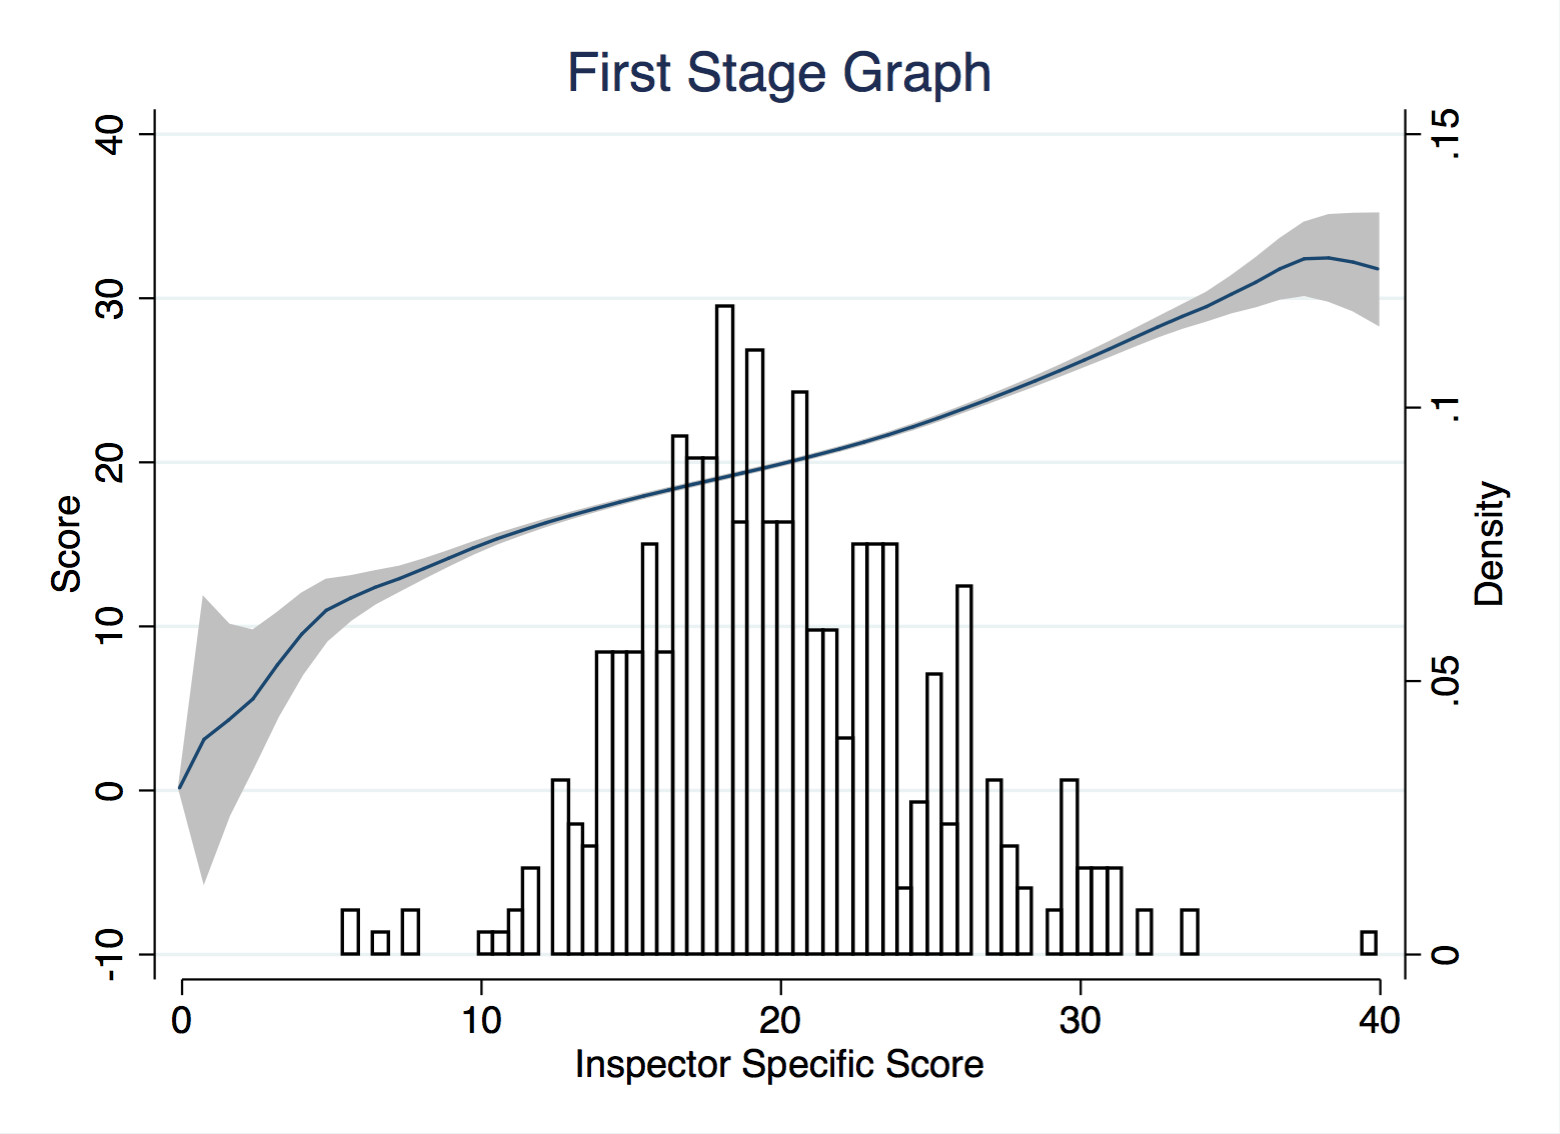
\includegraphics[scale = 0.35]{Figures/first_stage_score.png}
\caption{}
\footnotetext{The plot is generated based on 156,323 initial inspections conducted by inspectors who had done at least 50 initial inspections. The expected inspection score on the left y-axis is plotted against the leave-out average inspector scores on the x-axis. The right axis shows the density of inspector average scores.}
\label{first_stage_fig}
\end{figure}

\subsection{Impact of Inspection Scores on Subsequent Inspection Results}

In this section, I examine the effects of the inspection results on subsequent initial inspection results. I consider three outcomes of health inspections as the dependent variables: the overall score, whether the restaurant receives an A, and whether that restaurant gets temporally shutdown for a critical violation that it cannot correct by the end of the inspection. While the subsequent initial inspection's overall score offers a summary of the number of violations cited and the severities of those violations, the two other variables should also be of interest. Given the bunching of scores around the 13-14 threshold, we do not expect the treatment effect to be constant across different score ranges. In addition, increasing the proportion of initial inspections that result in As can reduce administrative costs for DOHMH by reducing the resources devoted to re-inspections. We should also examine temporary shutdowns since these are associated with critical violations that may pose the biggest threat to public health. 

To measure the effect of scores from initial inspections on subsequent initial inspection outcomes, I estimate the following equation: 
\begin{align}
        Y_{i,t^{next}} = \beta Score_{it} + \delta_i + \tau_{t} + \tau_{t^{next}} + \varepsilon_{it},
        \label{score}
\end{align}
where $Score_{i,t}$ is the score earned by restaurant $i$ on date $t$, $\delta_i$ and $\tau_t$ are the restaurant and date fixed effects, respectively, and $t^{next}$ is the date of the subsequent initial inspection. The error term $\varepsilon_{it}$ is two-way clustered at the inspector and zipcode levels. The term $Score_{it}$ is endogenous, so I instrument for it using the following first stage equation:
\begin{align}
score_{it} = \gamma Z_{it} + \delta_i + \tau_t + \epsilon_{it}
\label{first_stage_eq}
\end{align}
where $Z_{it}$ is defined in \eqref{instrument}.

Table \ref{Shutdown_A} reports the results. Given that the standard deviation of scores are around 14, the result suggests that one standard deviation increase in inspection scores increases the chance of getting an A during next initial inspection by about 3\%, which is almost a 10\% increase relative to the average 36\%. And one standard deviation increase in score decreases the chance of getting closed [TODO: More discussion here.]
\begin{table}
\centering
\scalebox{0.7}{\begin{tabular}{lcccccc} \hline
 & (1) & (2) & (3) & (4) & (5) & (6) \\
VARIABLES & Score (OLS) & Score (IV) & Closure (OLS) & Closure (IV) & Grade A (OLS) & Grade A (IV) \\ \hline
 &  &  &  &  &  &  \\
Score & -0.139*** & -0.242*** & -0.000763*** & -0.00101*** & -8.49e-05 & 0.00222*** \\
 & (0.00492) & (0.0162) & (8.26e-05) & (0.000185) & (0.000127) & (0.000556) \\
 &  &  &  &  &  &  \\
Observations & 149,831 & 149,831 & 138,674 & 138,674 & 149,831 & 149,831 \\
Inspection Date FE & YES & YES & YES & YES & YES & YES \\
Restaurant FE & YES & YES & YES & YES & YES & YES \\
 dependent mean & 21.08 & 21.08 & 0.0162 & 0.0162 & 0.372 & 0.372 \\ \hline
\multicolumn{7}{c}{ Robust standard errors in parentheses} \\
\multicolumn{7}{c}{ *** p$<$0.01, ** p$<$0.05, * p$<$0.1} \\
\end{tabular}
}
\caption{Impact of Inspection Scores on Temporary Closure and Obtaining Grade A}
\label{Shutdown_A}
\footnotetext{Standard errors are two-way clustered at zipcode and inspector levels.}
\end{table}

\subsection{Multi-task}

\begin{figure}[htbp]
\centering
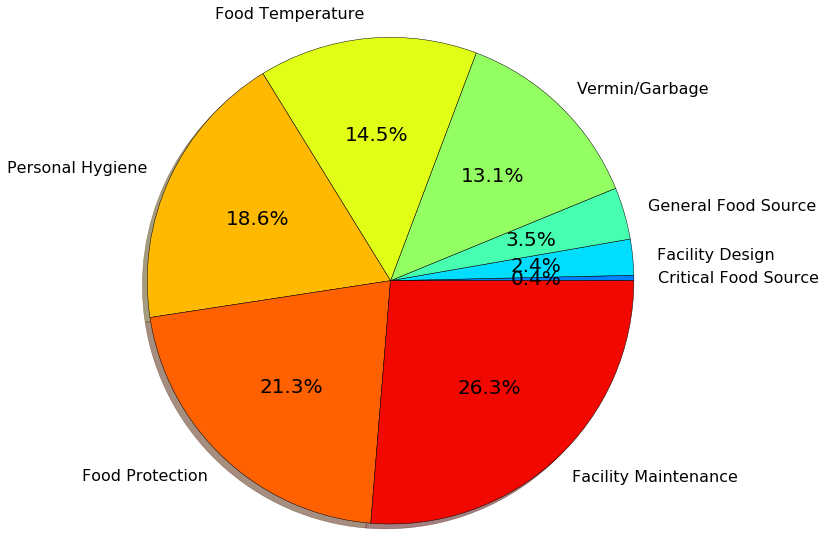
\includegraphics[scale = 0.3]{Figures/viol_group_pie.png}
\caption{Breakdown of Frequencies of Violation Groups}
\label{task_pie}
\end{figure}

So far, I have used the total score as an one dimensional summary of the inspection results. However, cleanliness is a multi-dimensional task. There are 82 violation codes, grouped into eight categories: food temperature, food source, food protection, facility design, personal hygiene, vermin, and facility maintenance. Figure \ref{task_pie} provides a visual breakdown of the frequencies by which these groups are cited. I measure the result of an inspection using an eight-dimensional binary vector. Each element of the vector represents one of the eight violation groups and encodes whether that inspection had at least one citation within that group. 

I test how restaurants' effort allocation responds to the citation profile using the following regression. 
\begin{align}
\label{multi_second}
    Pr(Cited_{igt^{next}}) = \sum_{g' \in \mathcal{G}} \beta_{gg'} Cited_{igt} + \delta X_i + \tau_t + \varepsilon_{igt},
\end{align}
where $Cited_{igt}$ is an indicator for whether restaurant $i$ receives a citation of violation in group $g$ on date $t$, $\tau_t$ is the date fixed effect and $X_i$ is the restaurant controls. As before, $Cited$ is an endogenous, so need to instrument it using inspector propensity. The coefficient $\beta_{gg'}$ measures how a restaurant's effort in group $g$ responds to a citation in group $g'$. To instrument eight endogenous variables, I construct each inspector's tendency to cite at least one violation in group $g$ by using a leave-out strategy similar to the one done in section \ref{IV}. More specifically, I construct the instrument of inspector $j$'s tendency to cite group $g$ at restaurant $i$ as
\begin{align*}
  Z_{ijg} = \frac{1}{n_j - n_{ij}} \left(\sum_{kjgt \neq ijgt} Cited_{ijgt}\right),
\end{align*}
where $n_j$ is the number of inspections made by inspector $j$ and $n_{ij}$ is the number of inspections inspector $i$ has made at restaurant $j$. The first stage is a system of equations defined as
\begin{align}
\label{multi_first}
    Pr(Cited_{ijgt}) = \sum_{g'\in \mathcal{G}} \theta_{gg'}Z_{ijg'} + \varepsilon_{ijgt}, 
\end{align}
where $\mathcal{G}$ is the set of violation groups. 

Table \ref{multi_second_reg} presents the results of \eqref{multi_second} instrumenting with \eqref{multi_first}. We see that the diagonal coefficients are all negative, and six of the eight groups are statistically significant at 90\% level. I find that restaurants improve the most in the areas of Facility Maintenance in response to citations in the same area, with one more citation leading to a 0.236 fewer expected citations in the subsequent inspection. 

\begin{table}[htbp]
\centering
\scalebox{0.54}{\begin{tabular}{lcccccccc} \hline
 & (1) & (2) & (3) & (4) & (5) & (6) & (7) & (8) \\
VARIABLES & Facility Maintenance & Food Protection & Personal Hygiene & Food Temperature & Vermin/Garbage & Gen. Food Source & Facility Design & Crit. Food Source \\ \hline
 &  &  &  &  &  &  &  &  \\
Facility Maintenance & \textcolor{red}{-0.236***} & 0.00733 & 0.000184 & -0.00506 & -0.000922 & -0.00159 & 0.000981 & -0.000509 \\
 & (0.00961) & (0.0119) & (0.0107) & (0.00944) & (0.00766) & (0.00380) & (0.00295) & (0.00140) \\
Food Protection & \textcolor{blue}{-0.0776**} & \textcolor{red}{-0.177***} & -0.00731 & -0.0142 & \textcolor{blue}{-0.0397*} & -0.0100 & 0.00372 & \textcolor{brown}{0.00780*} \\
 & (0.0378) & (0.0306) & (0.0410) & (0.0253) & (0.0227) & (0.0113) & (0.0108) & (0.00400) \\
Personal Hygiene & 0.0222 & -0.00484 & \textcolor{red}{-0.189***} & -0.00771 & -0.000551 & 0.00458 & 0.00129 & 0.00217 \\
 & (0.0156) & (0.0103) & (0.0148) & (0.00957) & (0.00892) & (0.00489) & (0.00320) & (0.00173) \\
Food Temperature & 0.0148 & -0.0261 & 0.0133 & \textcolor{red}{-0.214***} & -0.00923 & 0.00613 & -0.00622 & -0.00153 \\
 & (0.0216) & (0.0163) & (0.0162) & (0.0134) & (0.0128) & (0.00722) & (0.00573) & (0.00243) \\
Vermin/Garbage & \textcolor{brown}{0.132***} & \textcolor{blue}{-0.0784*} & 0.00134 & 0.0446 & \textcolor{red}{-0.174***} & 0.0128 & -0.0105 & -0.00126 \\
 & (0.0439) & (0.0404) & (0.0544) & (0.0318) & (0.0283) & (0.0159) & (0.0138) & (0.00404) \\
Gen. Food Source & -0.0114 & -0.00139 & -0.0456 & -0.0103 & \textcolor{blue}{-0.0395*} & \textcolor{red}{-0.191***} & -0.0147 & -0.000895 \\
 & (0.0291) & (0.0348) & (0.0374) & (0.0334) & (0.0202) & (0.0199) & (0.00933) & (0.00395) \\
Facility Design & 0.0265 & \textcolor{blue}{-0.195**} & -0.00742 & 0.0168 & -0.0235 & 0.00421 & \textcolor{red}{-0.199***} & \textcolor{brown}{0.0169*} \\
 & (0.0787) & (0.0925) & (0.0776) & (0.0551) & (0.0612) & (0.0296) & (0.0239) & (0.00977) \\
Crit. Food Source & 0.274 & -0.284 & 0.279 & 0.125 & -0.0346 & -0.0233 & -0.0643 & \textcolor{red}{-0.185***} \\
 & (0.248) & (0.207) & (0.244) & (0.195) & (0.142) & (0.0848) & (0.0682) & (0.0298) \\
Observations & 149,831 & 149,829 & 149,831 & 149,829 & 149,829 & 149,831 & 149,829 & 149,831 \\
Dependent mean & 0.989 & 0.802 & 0.842 & 0.645 & 0.503 & 0.125 & 0.0694 & 0.0126 \\ \hline
\multicolumn{9}{c}{ Robust standard errors in parentheses} \\
\multicolumn{9}{c}{ *** p$<$0.01, ** p$<$0.05, * p$<$0.1} \\
\end{tabular}
}
\caption{}
\label{multi_second_reg}
\footnotetext{Standard errors are two-way clustered at zipcode and inspector levels.}
\end{table}

The signs of the diagonals shed insight on the production function of restaurant cleanliness. We see that many off-diagonal elements are negative and statistically significant, which suggests that a citation in one dimension leads to an improvement in another dimension. This finding makes sense in light of the fact that various dimensions may be complementary. One example of such complementarity is that a citation in Food Protection also reduces the expected number of citations from subsequent inspections in Facility Maintenance and Vermin/Garbage by -0.0776 and 0.0397, respectively. A citation in Food Protection may lead the restaurant to improve along this dimension, which might include fixing a broken thermometer (violation 10E) that improves the Facility Maintenance dimension or better maintaining contact surface (violation 10F) that makes the kitchen more vermin proof. 

\subsection{Impact of Inspection Results on 311 Complaint Calls}
\label{complaints_analysis}
The ultimate goal of any food inspection programs is to reduce food-borne illness, but directly studying food poisoning is difficult. This outcome variable suffers from under-reporting, and more severe cases that result in hospitalization, the origin of the illness cannot be traced back to a specific establishment. Food inspection results serve as a convenient proxy for restaurant cleanliness. A couple studies have found evidence of association between inspection results and the likelihood of food-borne illness outbreaks.\footnote{See \cite{Irwin_89} and \cite{petran_12} and \cite{petran_12_a}.} In this section, I use 311 complaint calls of restaurants to supplement the findings in my previous sections.

I transform the inspection level data to a restaurant-month level data where each observation represents a month for each restaurant between the first and last recorded inspection. For each month, I calculate the inspection score as the score from the most recent inspection. I estimate the following equation.
\begin{align}
\label{complaint}
    Pr(called_{it}) = \delta_i + \tau_t + \beta_0 Score_{it} + \beta_1 Month\_Since\_Inspection_{it} \nonumber \\
    + \beta_2 Month\_Since\_Inspection_{it} \times Score_{it} + \varepsilon_{it}
\end{align}
where $called_{it}$ a binary variable that equals one if DOHMH received at least one complaint call for restaurant $i$ in month $t$. For the IV regression, I again instrument the score using equation \eqref{first_stage_eq}. 

\begin{table}[htbp]
\centering
\scalebox{0.68}{\begin{tabular}{lcccccc} \hline
 & (1) & (2) & (3) & (4) & (5) & (6) \\
VARIABLES & Prob Call (OLS) & Prob Call (OLS) & Prob Call (OLS) & Prob Call (IV) & Prob Call (IV) & Prob Call (IV) \\ \hline
 &  &  &  &  &  &  \\
SCORE & -4.68e-05*** & -7.07e-06 & -9.04e-05*** & -8.93e-05* & -9.14e-05* & -6.12e-05 \\
 & (1.54e-05) & (1.57e-05) & (1.79e-05) & (4.76e-05) & (4.98e-05) & (6.16e-05) \\
Months Since Inspection &  & 0.000540*** & -1.94e-05 &  & 0.000498*** & 0.000739* \\
 &  & (3.73e-05) & (6.63e-05) &  & (4.33e-05) & (0.000434) \\
c.mon\_from\_inspect\#c.SCORE &  &  & 5.03e-05*** &  &  & -2.19e-05 \\
 &  &  & (5.81e-06) &  &  & (3.96e-05) \\
 &  &  &  &  &  &  \\
Observations & 1,223,207 & 1,223,207 & 1,223,207 & 1,223,207 & 1,223,207 & 1,223,207 \\
Year-Month FE & YES & YES & YES & YES & YES & YES \\
Restaurant FE & YES & YES & YES & YES & YES & YES \\
 Dependent Mean & 0.0145 & 0.0145 & 0.0145 & 0.0145 & 0.0145 & 0.0145 \\ \hline
\multicolumn{7}{c}{ Robust standard errors in parentheses} \\
\multicolumn{7}{c}{ *** p$<$0.01, ** p$<$0.05, * p$<$0.1} \\
\end{tabular}
}
\caption{Impact of Inspection Scores on the Probability of Receiving 311 Complaint Call}
\label{calls}
\footnotetext{Sample include inspections conducted by inspectors who have conducted at least 50 inspections of the same type. Standard errors are two-way clustered at zipcode and inspector levels.}
\label{complaint_table}
\end{table}

Table \ref{calls} presents the result of \eqref{complaint}. We see that getting a one standard deviation worse inspection score lowers the probability of a 311 call in a month by around 0.01\%, which is almost a 10\% reduction relative to the sample average of 1.45\%.  


\section{Conclusion and Discussion}

This paper combines multiple administrative level data from New York City to study how restaurants hygiene practices respond to citations given out during health inspections. While studying the causal link between citations and later behaviors is difficult when the citations are not randomly assigned, this paper overcomes this issue by creating a quasi experiment that uses the random assignment of inspectors with differing levels of stringency as an instrumental variable. I find evidence that restaurants respond to citations of health code violations by improving their sanitation qualities, measured by improved results during subsequent inspections and reduced frequencies of customer complaint calls.


\bibliographystyle{apa}

\bibliography{Biblio}



\end{document}
